% Décrire avec précision les fonctions et solutions techniques associées (JEE, JSF, JAVA, CDI, DAO, métier, etc).
\section{\textbf{Spécificités techniques}}

\subsection{\textbf{Méthodologie}}
	Étant donné le contexte de ce projet (faible évolution des demandes du client, consignes) la méthode choisie est plutôt traditionnelle qu'agile. Une méthode basée sur le cycle en V semble donc adaptée. 
	
\begin{figure}[htbp]
	\caption{\label{fig:CEV} Cycle en V}
	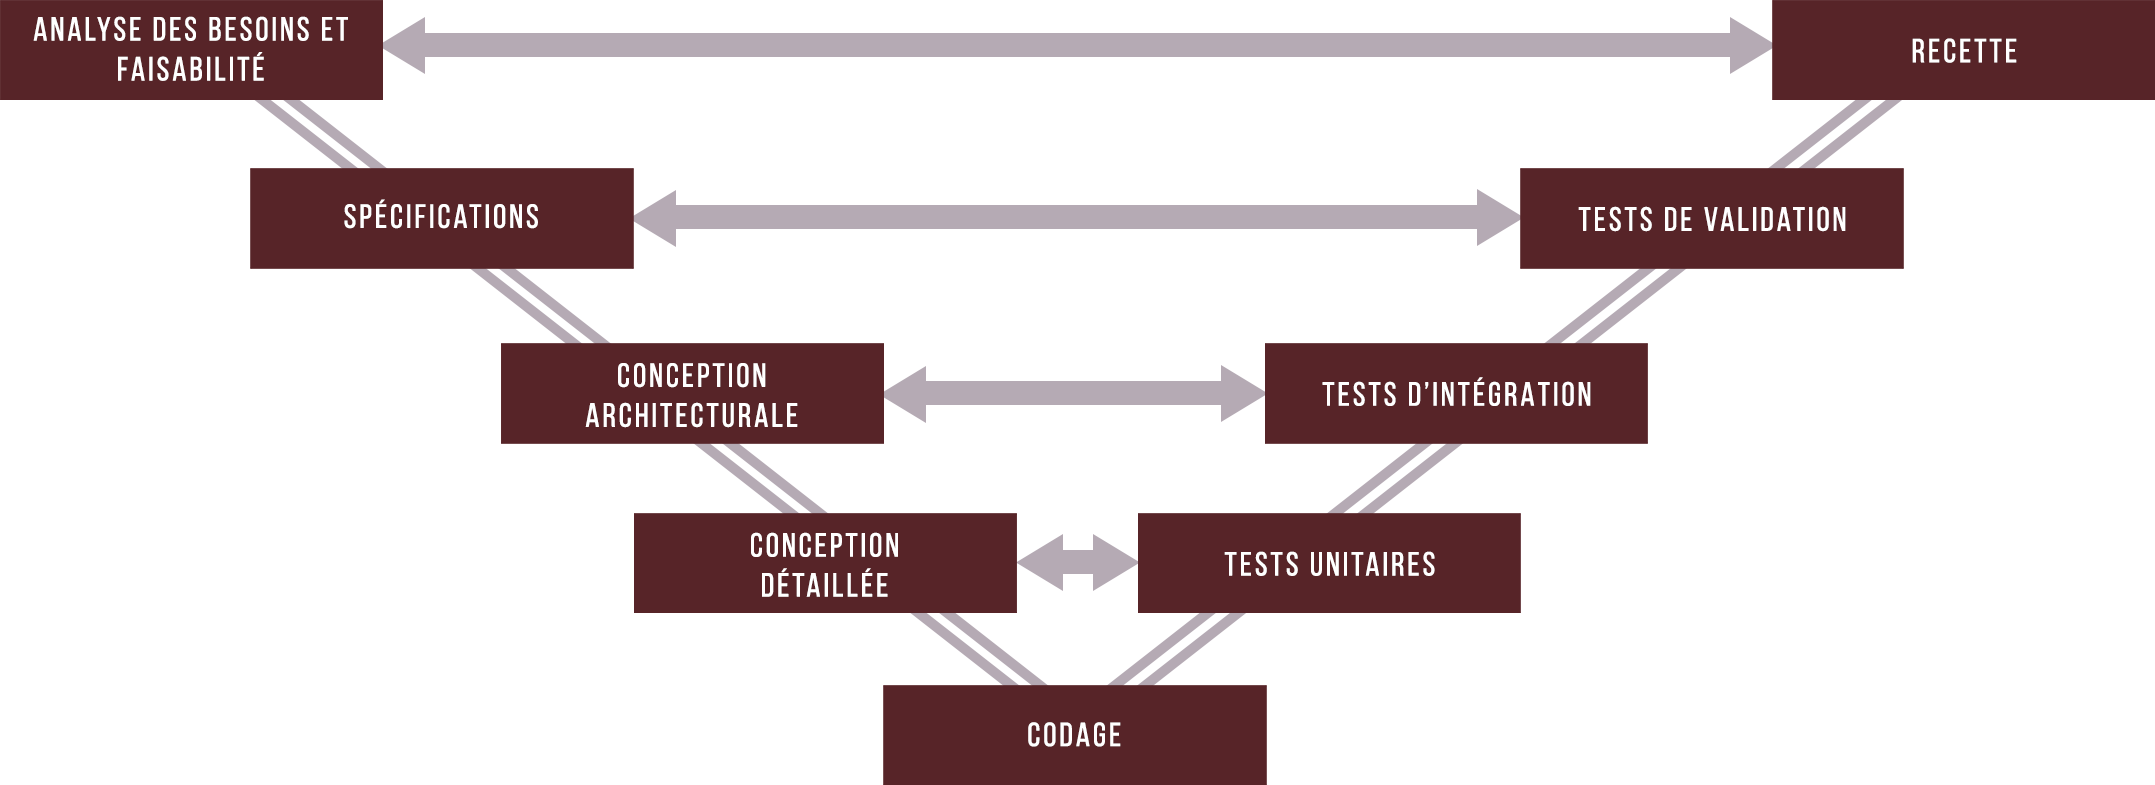
\includegraphics[width=1\textwidth]{CycleEnV.png}
\end{figure}

\subsection{\textbf{Architecture}}
	L'architecture de l'application 
	
\begin{figure}[htbp]
	\caption{\label{fig:CEV} Cycle en V}
	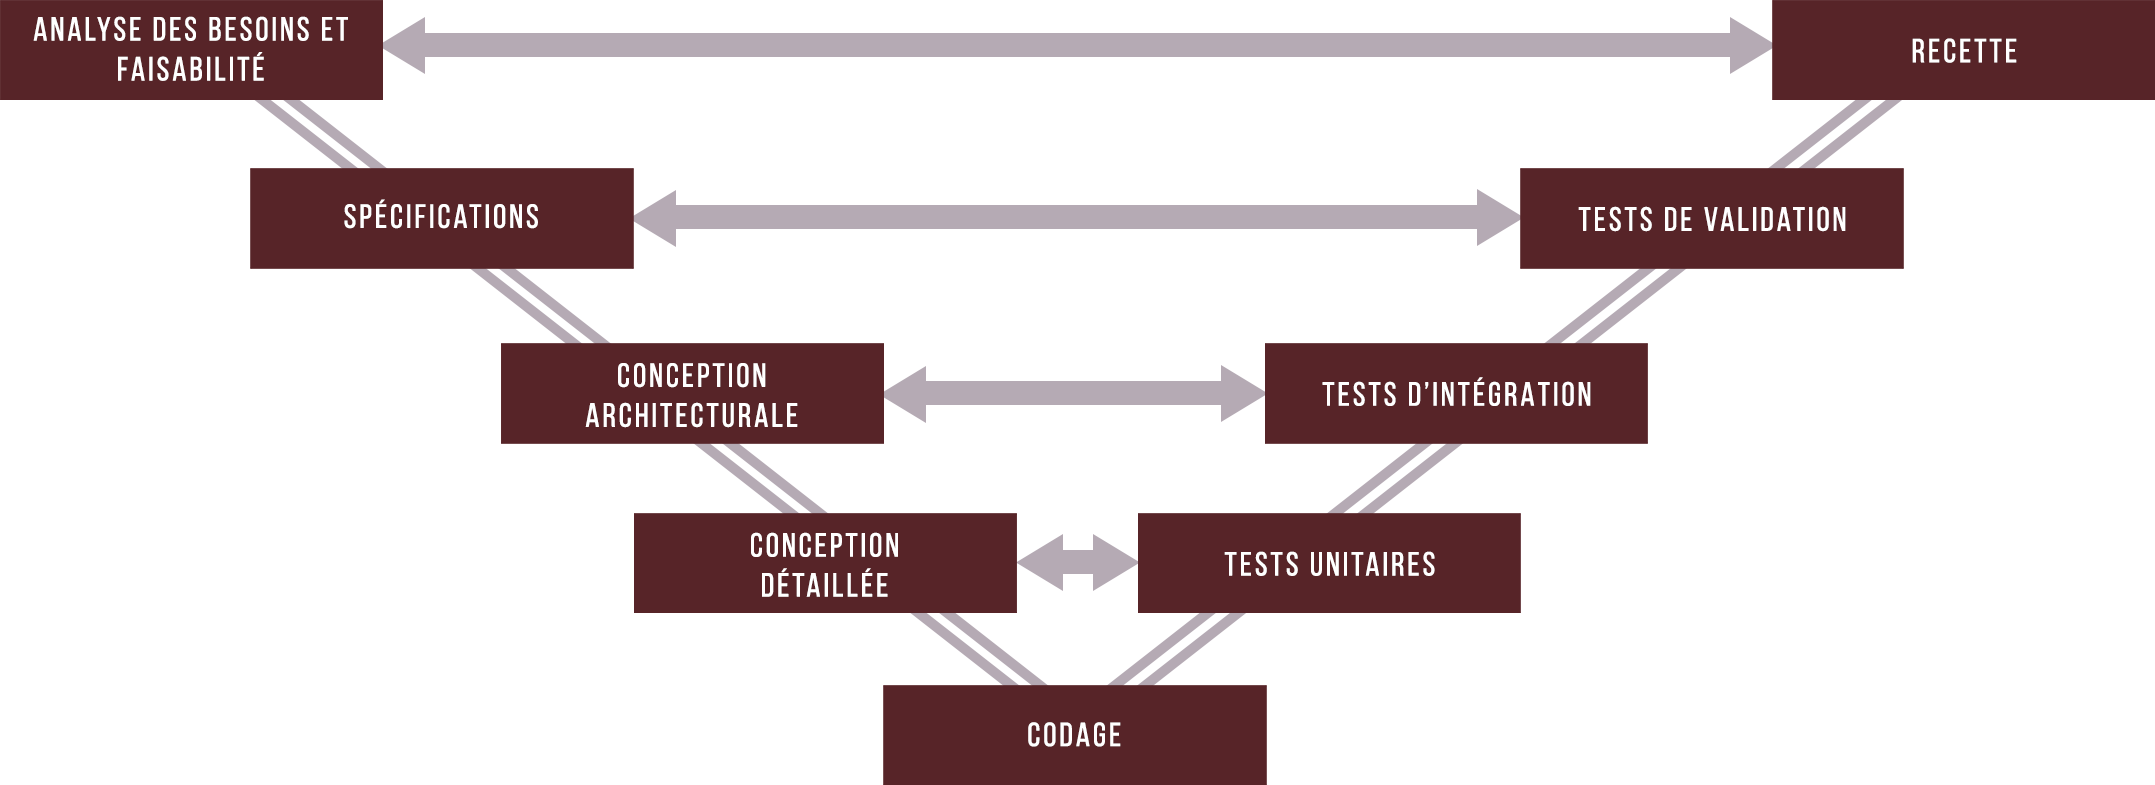
\includegraphics[width=1\textwidth]{CycleEnV.png}
\end{figure}
	
\subsection{\textbf{Langages}}
\noindent
% Tableau de trois cases de dimensions statiques séparées par des traits verticaux blancs
\begin{tabular}{!{\color{white}\vrule}m{3.4cm}!{\color{white}\vrule}m{1.7cm}!{\color{white}\vrule}m{10.8cm}!{\color{white}\vrule}}

% Trait horizontaux blancs
\arrayrulecolor{white}

\hline
% En-tête du tableau écrite en blanc sur fond rouge
\rowcolor{rougeBordeaux} \color{white} Nom & \color{white} Version & \color{white} Description\\

% Les lignes suivantes sont de couleurs alternées (gris clair / gris foncé)

\hline
\rowcolor{black!10} Java & - & Langage de programmation orienté objet.  \\

\hline
\rowcolor{black!20} HTML & - & Langage de balisage conçu pour représenter les pages web. \\

\hline
\rowcolor{black!10} CSS & - & Langage de feuille de style qui décrit la présentation des documents HTML et XML. \\

\hline
\rowcolor{black!20} XML & - & Langage qui permet de décrire des données à l'aide de balises et de règles personnalisables.  \\

\end{tabular}

\subsection{\textbf{Frameworks}}
\noindent
% Tableau de trois cases de dimensions statiques séparées par des traits verticaux blancs
\begin{tabular}{!{\color{white}\vrule}m{3.4cm}!{\color{white}\vrule}m{1.7cm}!{\color{white}\vrule}m{10.8cm}!{\color{white}\vrule}}

% Trait horizontaux blancs
\arrayrulecolor{white}

\hline
% En-tête du tableau écrite en blanc sur fond rouge
\rowcolor{rougeBordeaux} \color{white} Nom & \color{white} Version & \color{white} Description\\

% Les lignes suivantes sont de couleurs alternées (gris clair / gris foncé)
\hline
\rowcolor{black!10} Bootstrap & - & Collection d'outils utiles à la création du design (graphisme, animation et interactions avec la page dans le navigateur, etc.) de sites et d'applications web. \\

\hline
\rowcolor{black!20} JUnit & 5 & Framework de test unitaire pour le langage de programmation Java. \\

\hline
\rowcolor{black!10} Mockito & - & Framework Java permettant de générer automatiquement des objets ‘mockés‘. Facilite l’écriture des tests unitaires. \\

\hline
\rowcolor{black!20} Hibernate & - & Framework open source gérant la persistance des objets en base de données relationnelle. \\

\hline
\rowcolor{black!10} CDI & - & Framework standard d'injection de dépendances et de contextes, au sein de la plateforme Java et plus particulièrement Jakarta EE. \\

\hline
\rowcolor{black!20} JSF & - & Framework MVC Java basé sur la notion de composants, où leur état est enregistré lors du rendu de la page, pour être ensuite restauré au retour de la requête.   \\

\hline
\rowcolor{black!10} PrimeFaces & - & Framework open-source offrant une collection de composants d'interface pour JavaServer Faces.  \\

\hline

\end{tabular}

\subsection{\textbf{Outils divers}}
\noindent
% Tableau de trois cases de dimensions statiques séparées par des traits verticaux blancs
\begin{tabular}{!{\color{white}\vrule}m{3.4cm}!{\color{white}\vrule}m{1.7cm}!{\color{white}\vrule}m{10.8cm}!{\color{white}\vrule}}

% Trait horizontaux blancs
\arrayrulecolor{white}

\hline
% En-tête du tableau écrite en blanc sur fond rouge
\rowcolor{rougeBordeaux} \color{white} Nom & \color{white} Version & \color{white} Description\\

% Les lignes suivantes sont de couleurs alternées (gris clair / gris foncé)
\hline
\rowcolor{black!10} MySQL & - & Système de gestion de bases de données relationnelles (SGBDR). \\

\hline
\rowcolor{black!20} Tomcat & 8.5 & Conteneur web qui permet d'exécuter des applications web reposant sur les technologies servlets et JSP. \\

\hline
\rowcolor{black!10} EJB & - & Architecture de composants logiciels côté serveur pour la plateforme de développement Jakarta EE. \\

\hline
\rowcolor{black!20} JPA & - & Interface de programmation Java permettant de définir facilement des objets métier, qui pourront servir d'interface entre la base de données et l'application, dans le cadre d'un mapping objet-relationnel. Elle repose essentiellement sur l'utilisation d'annotations.  \\

\hline
\rowcolor{black!10} AJAX & - & Ensemble de technologies destinées à réaliser de rapides mises à jour du contenu d'une page Web, sans qu'elles nécessitent le moindre rechargement visible par l'utilisateur de la page Web. \\

\hline

\end{tabular}

\subsection{\textbf{Logiciels et Applications web}}
\noindent
% Tableau de trois cases de dimensions statiques séparées par des traits verticaux blancs
\begin{tabular}{!{\color{white}\vrule}m{3.4cm}!{\color{white}\vrule}m{1.7cm}!{\color{white}\vrule}m{10.8cm}!{\color{white}\vrule}}

% Trait horizontaux blancs
\arrayrulecolor{white}

\hline
% En-tête du tableau écrite en blanc sur fond rouge
\rowcolor{rougeBordeaux} \color{white} Nom & \color{white} Version & \color{white} Description\\

\hline
\rowcolor{black!10} PhpMyAdmin & - & Application web permettant de gérer une base de données MySQL sur un serveur PHP facilement. \\

\hline
\rowcolor{black!20} Eclipse JEE & 2019-XX & Environnement de développement pour réaliser des applications Jakarta EE et Web. \\

\hline
\rowcolor{black!10} Git / GitHub & - & Git est un logiciel de gestion de versions décentralisé et GitHub le service web d'hébergement et de gestion de développement associé. \\

\hline

\end{tabular}

\subsection{\textbf{Base de données}}
	Une base de données est nécessaire afin de faire persister les personnes ainsi que leur CV. Le modèle conceptuel des données ci dessous représente son l'architecture.